\section{Comparison to State-of-the-art}\label{sec:vs_clsmith}

In this section we report on an experiment using both CLSmith and CLgen for 48 hours each.

Total runtime for a test cases consists of the generation time, the time to execute the test harness on a configuration, and, if required, the time to reduce the test case.

Both testing frameworks were used for 48 hours each. CLSmith was configured with default settings. CLReduce was configured with the default settings (four parallel reduction threads).

\subsection{Experimental Setup}

Each device was configured to run the compiler testing system for a fixed 48 hours. All devices were otherwise unloaded.

\subsection{Results}

Table~\ref{tab:outcomes} shows the outcomes of test cases. Column \textbf{bc} is of immediate value for developers; for all other outcomes, differential testing is required.

Once voting heuristics have been applied, the result is table~\ref{tab:classifications}.

\begin{table*}
	\scriptsize %
	\centering %
	  \begin{tabular}{lll | rrrrrrr | rrrrrrr }
  \toprule
  & & & \multicolumn{7}{c|}{\textbf{CLSmith}} & \multicolumn{7}{c}{\textbf{CLgen}} \\
  \textbf{\#.} & \textbf{Device} & $\pm$ &
  \textbf{bf} & \textbf{bc} & \textbf{bto} & \textbf{c} & \textbf{to} & \cmark & \textbf{total} &
  \textbf{bf} & \textbf{bc} & \textbf{bto} & \textbf{c} & \textbf{to} & \cmark & \textbf{total} \\
  \midrule
  \multirow{ 2}{*}{1} & \multirow{ 2}{*}{GeForce GTX 1080} & $-$ & 375 & 0 & 3 & 68 & 423 & 4267 & 5136       & 20063 & 13 & 0 & 910 & 42 & 8116 & 29144 \\& & $+$ & 404 & 0 & 0 & 44 & 517 & 4586 & 5551 & 22958 & 13 & 0 & 789 & 36 & 6720 & 30516 \\
\hline
\multirow{ 2}{*}{2} & \multirow{ 2}{*}{GeForce GTX 780} & $-$ & 488 & 12 & 3 & 16 & 620 & 5567 & 6706       & 10593 & 18 & 141 & 1059 & 124 & 10116 & 22051* \\& & $+$ & 504 & 0 & 0 & 32 & 658 & 5689 & 6883 & 10679 & 18 & 131 & 1091 & 112 & 10020 & 22051* \\
\hline
\multirow{ 2}{*}{3} & \multirow{ 2}{*}{Intel HD Haswell GT2} & $-$ & 166 & 938 & 894 & 0 & 0 & 269 & 2267       & 33838 & 215 & 60 & 2474 & 0 & 22049 & 58636 \\& & $+$ & 165 & 939 & 893 & 0 & 0 & 265 & 2262 & 26684 & 183 & 59 & 1506 & 0 & 20283 & 48715* \\
\hline
\multirow{ 2}{*}{4} & \multirow{ 2}{*}{Intel E5-2620 v4} & $-$ & 1103 & 173 & 22 & 513 & 448 & 4858 & 7117       & 35858 & 94 & 38 & 2205 & 82 & 13327 & 51604 \\& & $+$ & 1051 & 0 & 4 & 493 & 592 & 4586 & 6726 & 34068 & 53 & 0 & 2284 & 152 & 13554 & 50111 \\
\hline
\multirow{ 2}{*}{5} & \multirow{ 2}{*}{Intel E5-2650 v2} & $-$ & 412 & 35 & 63 & 68 & 477 & 4577 & 5632       & 10290 & 364 & 110 & 1216 & 60 & 10090 & 22130* \\& & $+$ & 483 & 0 & 3 & 8 & 623 & 5531 & 6648 & 10340 & 370 & 103 & 1232 & 81 & 10004 & 22130* \\
\hline
\multirow{ 2}{*}{6} & \multirow{ 2}{*}{Intel i5-4570} & $-$ & 1178 & 184 & 18 & 12 & 523 & 5792 & 7707       & 12027 & 452 & 120 & 1262 & 55 & 11722 & 25638* \\& & $+$ & 1065 & 0 & 2 & 9 & 640 & 5125 & 6841 & 14527 & 460 & 168 & 1257 & 87 & 14026 & 30525* \\
\hline
\multirow{ 2}{*}{7} & \multirow{ 2}{*}{Intel Xeon Phi} & $-$ & 134 & 10 & 503 & 0 & 105 & 1041 & 1793       & 8606 & 47 & 21 & 686 & 115 & 5781 & 15256 \\& & $+$ & 370 & 0 & 24 & 171 & 449 & 4020 & 5034 & 8621 & 38 & 3 & 671 & 140 & 5660 & 15133 \\
\hline
\multirow{ 2}{*}{8} & \multirow{ 2}{*}{Intel E5-2620 (POCL)} & $-$ & 468 & 0 & 2 & 15 & 585 & 5351 & 6421       & 31564 & 39 & 0 & 2478 & 40 & 9834 & 43955 \\& & $+$ & 486 & 0 & 0 & 64 & 602 & 5541 & 6693 & 31209 & 40 & 0 & 2405 & 62 & 8973 & 42689 \\
\hline
\multirow{ 2}{*}{9} & \multirow{ 2}{*}{Intel E5-2620 (ComputeAorta)} & $-$ & 493 & 0 & 0 & 200 & 668 & 5722 & 7083       & 10801 & 698 & 105 & 359 & 17 & 10145 & 22125* \\& & $+$ & 409 & 0 & 0 & 5 & 569 & 4873 & 5856* & 10855 & 816 & 124 & 318 & 12 & 10000 & 22125* \\
\hline
\multirow{ 2}{*}{10} & \multirow{ 2}{*}{Oclgrind Simulator} & $-$ & 142 & 0 & 0 & 0 & 188 & 1623 & 1953       & 33246 & 2309 & 0 & 1084 & 279 & 10691 & 47609 \\& & $+$ & 140 & 0 & 0 & 0 & 190 & 1587 & 1917 & 31357 & 2182 & 0 & 1046 & 298 & 10346 & 45229 \\
  \bottomrule
\end{tabular}


	\caption{Test case outcomes using CLSmith and CLgen for 24 hours each. Configuration \#. as per Table~\ref{tab:platforms}. $\pm$ denotes optimizations off ($-$) vs on ($+$). The remaining columns denote build failure (\textbf{bf}), build crash (\textbf{bc}), build timeout (\textbf{bto}), runtime crash (\textbf{c}), timeout (\textbf{to}), and passed (\textbf{\cmark}) outcomes for CLSmith and CLgen, respectively. \cc{Asterisk in 'total' column means incomplete data. All results are excluding reductions.}}
	\label{tab:outcomes}
\end{table*}

\begin{table*}
	\scriptsize %
	\centering %
	\begin{tabular}{lll | rrrrr | rrrrr }
  \toprule
  & & & \multicolumn{5}{c|}{\textbf{CLSmith}} & \multicolumn{5}{c}{\textbf{CLgen}} \\
  \textbf{\#.} & \textbf{Device} & $\pm$ &
  \textbf{w} & \textbf{bf} & \textbf{c} & \textbf{to} & \textbf{\% of total} &
  \textbf{w} & \textbf{bf} & \textbf{c} & \textbf{to} & \textbf{\% of total} \\
  \midrule
  \multirow{ 2}{*}{1} & \multirow{ 2}{*}{GeForce GTX 1080} & $-$ & 0 & 0 & 17 & 25 & 0.8\%       & 10 & 45 & 28 & 5 & 0.4\% \\& & $+$ & 5 & 0 & 63 & 15 & 1.5\% & 14 & 28 & 12 & 14 & 0.3\% \\
\hline
\multirow{ 2}{*}{2} & \multirow{ 2}{*}{GeForce GTX 780} & $-$ & 3 & 0 & 22 & 37 & 0.9\%       & 617 & 406 & 65 & 42 & 25.9\% \\& & $+$ & 0 & 0 & 10 & 37 & 0.7\% & 281 & 375 & 37 & 68 & 22.9\% \\
\hline
\multirow{ 2}{*}{3} & \multirow{ 2}{*}{Intel HD Haswell GT2} & $-$ & 0 & 0 & 0 & 0 & 0.0\%       & 108 & 473 & 20 & 0 & 1.2\% \\& & $+$ & 0 & 0 & 0 & 0 & 0.0\% & 22 & 39 & 6 & 0 & 0.2\% \\
\hline
\multirow{ 2}{*}{4} & \multirow{ 2}{*}{Intel E5-2620 v4} & $-$ & 0 & 563 & 192 & 0 & 11.2\%       & 3 & 10 & 93 & 1 & 0.3\% \\& & $+$ & 0 & 595 & 434 & 1 & 14.5\% & 1 & 7 & 110 & 3 & 0.3\% \\
\hline
\multirow{ 2}{*}{5} & \multirow{ 2}{*}{Intel E5-2650 v2} & $-$ & 0 & 0 & 0 & 0 & 0.0\%       & 2 & 65 & 131 & 1 & 23.9\% \\& & $+$ & 0 & 0 & 61 & 0 & 1.1\% & 8 & 66 & 138 & 3 & 25.1\% \\
\hline
\multirow{ 2}{*}{6} & \multirow{ 2}{*}{Intel i5-4570} & $-$ & 0 & 570 & 0 & 0 & 8.3\%       & 15 & 362 & 156 & 10 & 20.2\% \\& & $+$ & 0 & 629 & 0 & 0 & 8.2\% & 6 & 167 & 170 & 10 & 31.6\% \\
\hline
\multirow{ 2}{*}{7} & \multirow{ 2}{*}{Intel Xeon Phi} & $-$ & 6 & 0 & 131 & 5 & 2.8\%       & 19 & 30 & 0 & 73 & 0.9\% \\& & $+$ & 1 & 0 & 0 & 4 & 0.3\% & 12 & 32 & 0 & 65 & 0.8\% \\
\hline
\multirow{ 2}{*}{8} & \multirow{ 2}{*}{POCL (Intel E5-2620)} & $-$ & 0 & 0 & 56 & 2 & 0.9\%       & 2 & 6 & 850 & 7 & 2.8\% \\& & $+$ & 0 & 0 & 8 & 18 & 0.4\% & 1 & 7 & 930 & 1 & 2.9\% \\
\hline
\multirow{ 2}{*}{9} & \multirow{ 2}{*}{ComputeAorta (Intel E5-2620)} & $-$ & 0 & 0 & 0 & 11 & 0.2\%       & 15 & 620 & 85 & 0 & 38.8\% \\& & $+$ & 9 & 0 & 177 & 35 & 3.1\% & 19 & 563 & 49 & 6 & 39.4\% \\
\hline
\multirow{ 2}{*}{10} & \multirow{ 2}{*}{Oclgrind Simulator} & $-$ & 0 & 0 & 0 & 8 & 0.4\%       & 6 & 3 & 13 & 80 & 0.3\% \\& & $+$ & 0 & 0 & 0 & 14 & 0.7\% & 7 & 2 & 9 & 50 & 0.2\% \\
  \bottomrule
\end{tabular}


	\caption{Using voting heuristics to expose anomalous results in Table~\ref{tab:outcomes}. Columns denote wrong-code (w), build failure (\textbf{bf}), runtime crash (\textbf{c}), and timeout (\textbf{to}) classifications for CLSmith and CLgen, respectively. \cc{Asterisk in 'total' column means incomplete data. All results are excluding reductions.}}
	\label{tab:classifications}
\end{table*}

\cc{TODO: How long do reductions take? How many CLgen test cases can we run in that amount of time? Given the ratio of interesting CLgen test cases, how many more bugs could we find in the amount of time it takes to run a single reduction?}

\cc{TODO: We note that we tested the wrong-code classification of CLSmith, finding that it does not affect the number of CLSmith wrong-code bugs.}


\subsection{Analysis of bugs found}

For all except configuration $3\pm$, CLgen exposes more compiler crashes than CLSmith. On average, CLgen hangs the compiler more frequently.


\subsection{Test Case Size}

Median CLSmith kernel is 1086 lines long (excluding headers).

For ``interesting'' programs: median CLgen kernel size is 12 lines. Median reduced CLSmith kernel size is 43 lines (894 lines before reduction). Figure~\ref{fig:kernel-sizes}.

Potentially interesting questions: What is the total lines of code which get run on each device during the tests? CLgen programs are smaller, but we get through more of them.

\cc{CLgen test cases are two orders of magnitude smaller than CLSmith programs which have been reduced.}

\cc{What is the bug rate per line of code?}

\begin{figure}
	\centering %
	\includegraphics[width=\columnwidth]{build/img/runtimes}%
	\caption{%
		Test case runtimes, excluding timeouts. On average, CLgen test case execution is $x\times$ faster than CLSmith. \cc{TODO: CLgen generation times, CLgen reductions}%
	}%
	\label{fig:runtimes} %
\end{figure}


\begin{figure}
	\centering %
	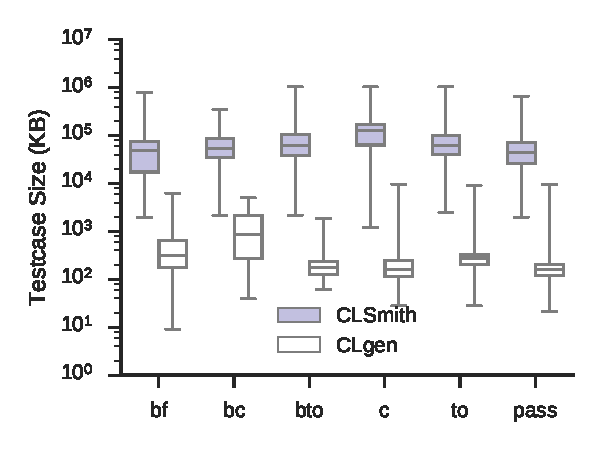
\includegraphics[width=\columnwidth]{build/img/kernel-sizes}%
	\caption{%
		Kernel line counts, grouped by classification. CLSmith programs with wrong-code (\emph{w}) classifications have been reduced.%
	}%
	\label{fig:kernel-sizes} %
\end{figure}


\begin{figure}
	\centering %
	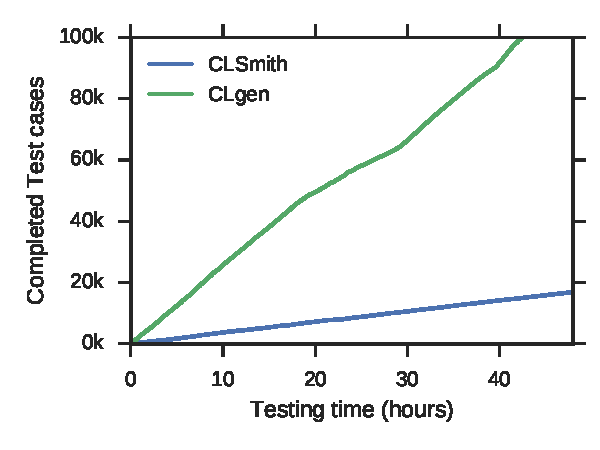
\includegraphics[width=\columnwidth]{build/img/total-tests}%
	\caption{%
		Test cases. \cc{TODO: Replot with the fastest and slowest device for each}%
	}%
	\label{fig:total-tests} %
\end{figure}